% Arabic version of the CN2 paper.
% Compile with: lualatex (polyglossia + bidi via luabidi).
% Tables and the algorithm are wrapped in \begin{english} for robust RTL handling.
\documentclass[12pt]{article}

\usepackage{polyglossia}
\usepackage[margin=1in]{geometry}
\usepackage{amsmath,amssymb,amsthm}
\usepackage{booktabs}
\usepackage{graphicx}
\usepackage{hyperref}
\usepackage[ruled,vlined]{algorithm2e}
\usepackage{xcolor}
\usepackage{float}
\usepackage{enumitem}

% ---- Arabic font selection ----
\setmainlanguage{arabic}
\setotherlanguage{english}
\newfontfamily\arabicfont[Script=Arabic]{Amiri}
\newfontfamily\arabicfontsf[Script=Arabic]{Amiri}

\SetKwRepeat{كرر حتى}{كرر}{حتى}

\newtheorem{theorem}{نظرية}
\newtheorem{lemma}{تمهيدية}
\newtheorem{definition}{تعريف}
\newtheorem{assumption}{افتراض}

\newcommand{\R}{\mathbb{R}}
\newcommand{\lam}{\lambda}
\newcommand{\grad}{\nabla}
\newcommand{\cn}{CN^2}

\title{\textbf{نيوتن--نيستيروف المُتابَع بالنقاط ($\cn$):\\ إطار تبادل مرحلي للتحسين الهجين من الرتبتين الأولى والثانية}}
\author{جيجي\; والزملاء\\[2mm]{\textenglish{Jay \& Collaborators}}}
\date{\today}

\begin{document}
\maketitle

\begin{abstract}
نقترح إطار تبادل مرحلي اسمه \emph{نيوتن--نيستيروف المُتابَع بالنقاط} ($\cn$)، يتناوب بين
طور \emph{تدرّج نيستيروف المتسارع} (NAG) الخام وطور \emph{نيوتن} المحلي. بدل أن نمزج الزخم
بمعلومات الإنحناء باستمرار (كما في أساليب نيوتن التكعيبية القصورية الحديثة)، يؤدّي $\cn$
تبديلاً \emph{قسريّاً}: عندما يدل انحطاط نيوتن $\lam(x)$ على تجاوز حوض الحلّ، نتنقّل بخطوات
متسارعة رخيصة من الرتبة الأولى؛ وعندما يهبط الانحطاط دون عتبة المستخدم $\tau$، نلتزم
بنيوتن المُخمّد للحصول على تقارُب تربيعي محلي. في المناطق غير المحدّبة حيث لا يكون
هيسيان موجب التحدد، نلجأ إلى بوابة معيار التدرج، مما يجعل الطريقة قوية على دوالّ مثل
Rosenbrock وBeale حيث يفشل نيوتن الخام فجأة. في مجموعة من المسائل الاختبارية يتقارب $\cn$
في كل حالة، بما فيها Rosenbrock في البعد $n=200$ حيث يعلَّق كلٌّ من نيوتن وNewton-CG وL-BFGS،
مع عدد مماثل أو أقل من تقييمات الهيسيان. الطريقة متينة على الوسيط المستخدم $K_0$ (طول
الوثبة) وتكشف مفاضلة دقة-تكلفة نظيفة في العتبة $\tau$.
\end{abstract}

\section{مقدمة}
\label{sec:intro-ar}

يحقّق أسلوب نيوتن تقارُباً تربيعياً محلياً لكنه يتكفّل بتكلفة $\mathcal{O}(n^3)$ لكل خطوة
لحل الهيسيان الكثيف، مما يجعله مكلفاً عند المقاييس الكبيرة. وتحقق طرق التدرج المتسارع
لنيستيروف (NAG) المعدّل الأمثل $\mathcal{O}(1/k^2)$ للمسائل المحدّبة الملساء لكنها تتباطأ
هندسياً قرب الحل، خاصّة في الأهداف سيئة التكييف. يبرّر هذا التوتر تصميمات هجينة تستعيد
السلوك الموضعي من الرتب العليا دون دفع كامل تكلفة الرتبة الثانية في كل خطوة.

ركّزت الأعمال الأخيرة على \emph{المزج المستمر} بين الزخم والتنظيم التكعيبي، مثل نيوتن
التكعيبي القصوري (ICN)~\cite{icn2026}، وطرق نيوتن التكعيبية المتسارعة~\cite{optami2025}،
وطرق التكعيبية العشوائية المعزّزة بالزخم~\cite{aistats2025}. تمزج هذه الأساليب الزخم
بالانحناء على أساس كل خطوة. وفي المقابل، ندرس هنا تصميماً أدقّ وأكثر تفسيرية: نبقي
العائلتين الحسابيتين \emph{منفصلتين} ونتبدّل بينهما فقط عند \emph{نقاط تتبّع} خشنة
(checkpoints). هذه فلسفة ``التنقّل من الخشن إلى الدقيق'': تُدقَّق تقييمات نيوتن المكلفة
نادراً، وتملأ خطوات التدرج المتسارع الفجوات.

مساهمتنا طريقة \emph{مرحلية} مبدئية:
\begin{enumerate}
\item تشغيل دفعة نيوتن قصيرة (خطوتي مخمّدَتين) وتقييم انحطاط نيوتن؛
\item إذا تجاوز الانحطاط عتبةً (أي نحن بعيدون عن الحل)، تشغيل طور نيستيروف حتى
      يدخل الانحطاطُ المقياسُ بإيقاع هيسيان نادر متكيّف مع البعد حوضَ الحل؛
\item اللجوء إلى بوابة معيار التدرج في المناطق غير المحدّبة حيث الهيسيان ليس موجب
      التحدد، بما يضمن متانةً عالمية.
\end{enumerate}

\section{الخوارزمية $\cn$}
\label{sec:method-ar}

نصغّر دالةً ملساء (ربما غير محدّبة) $f:\R^n\to\R$. ليكن $\grad f$ التدرج و
$H=\grad^2 f$ الهيسيان. \emph{انحطاط نيوتن} هو
\begin{equation}
\label{eq:lambda-ar}
\lam(x)=\sqrt{\grad f(x)^{\top}\big(H(x)+\rho I\big)^{-1}\grad f(x)},
\end{equation}
حيث $\rho\ge0$ إزاحة تنظيمية صغيرة. في المسائل المحدّبة ذات $H\succ 0$, يكون $\lam(x)$
مقياسَ قربٍ طبيعياً للحل.

\textbf{البوابة المزدوجة.} عندما لا يكون $H$ موجب التحدد (منطقة غير محدّبة)، لا يعود
الانحطاط (1) ذا معنى. لذلك نعرّف مقياس الدخول
\begin{equation}
g(x)=\begin{cases}
\lam(x), & H(x)\succ 0,\\[2mm]
\|\grad f(x)\|, & \text{غير ذلك},
\end{cases}
\end{equation}
ونقارنه بعتبة $\tau$ (لحالة الهيسيان) أو $\tau_g$ (للتدرج). هذه البوابة المزدوجة (الخيار
``جـ'') هي ما يجعل الطريقة متينةً على دوالّ غير محدّبة مثل Rosenbrock وBeale.

\begin{algorithm}[H]
\caption{$\cn$ (نيوتن--نيستيروف المُتابَع بالنقاط)}
\label{alg:cn2-ar}
\begin{english}\small
\KwIn{$x_0$, thresholds $\tau,\tau_g>0$, jump length $K_0$, Newton steps $m=2$.}
\Repeat{the entry measure falls below the threshold}{
  run $m$ damped-Newton steps, each with a fresh Hessian\;
  compute the entry measure $g(x)$ from a fresh Hessian\;
  \If{$g(x)\le$ threshold}{\Return converged at $x$\;}
  run $K_0$ Nesterov steps with backtracking, re-checking $g(x)$ every
  $K_{ck}=\max(20,\lfloor n/5\rfloor)$ steps (fresh Hessian)\;
}
\end{english}
\end{algorithm}

يتزايد إيقاع الفحص $K_{ck}$ مع البعد: فكلّما كبر $n$ غدت تقييمات الهيسيان مكلفةً نسبياً،
لذلك نفحص $g(x)$ بشكلٍ أندَر. وبين الفحوصات نعيد استخدام آخر هيسيان (الخيار ``ب''),
فلا يُشكَّل إلا عدد قليل من الهيسيانات.

\section{التقارب}
\label{sec:theory-ar}

نحتاج الافتراضات المعيارية التالية.

\begin{assumption}[الملاسة]
\label{asm:smooth-ar}
$f$ قابلة للاشتقاق مرتين بتدرج Lipschitz من ثابت $L$, وهيسيانها يحقق
$\|H(x)-H(y)\|\le M\|x-y\|$ على مجموعة المستوى الفرعي $\{x:f(x)\le f(x_0)\}$.
\end{assumption}

\begin{assumption}[الانحناء في حوض الحل]
\label{asm:conv-ar}
$f$ محدّبة قوياً بثابت $\mu$ في \emph{حوض الحل} $\Omega=\{x:\lam(x)\le \tau\}$، أي
$H(x)\succeq \mu I$ لكل $x\in\Omega$.
\end{assumption}

\begin{theorem}[دخول حوض الحل]
\label{thm:enter-ar}
ليتحقق الافتراض~\ref{asm:smooth-ar}. إذا تقارَب طور نيستيروف (بمعنى زوال التدرجات تباعاً)
أو فحص إيقاعُ الهيسيان نقطةً $x$ مقياسَ دخولها $g(x)\le \tau$ (أو $\tau_g$)، فإن
الخوارزمية~\ref{alg:cn2-ar} تدخل $\Omega$ وتنتقل إلى طور نيوتن.
\end{theorem}

\begin{proof}
(مخطط.) في ظل الافتراض~\ref{asm:smooth-ar}, تكون خطوة NAG بالتدرّج الخلفي خطوةً تنازلية
تخفض $f$ بمقدار $\tfrac12\alpha\|\grad f\|^2$. فإذا طال طور NAG دون خروجٍ مبكّر، يضمحل
معيار التدرج ويُفعَّل في النهاية معيار بوابة التدرج $\|\grad f\|\le\tau_g$ (أو يكشف
هيسيانٌ مفحوصٌ أن $\lam\le\tau$). عند تلك اللحظة نكون في $\Omega$ ويتولّى طور نيوتن.
\end{proof}

\begin{theorem}[التقارب التربيعي المحلي]
\label{thm:quad-ar}
ليتحقق الافتراضان~\ref{asm:smooth-ar} و~\ref{asm:conv-ar} ولأوصَل طور NAG نقطةً $x\in\Omega$
ذات $\lam(x)\le\tau$. حينها يتقارب طور نيوتن المخمّد تربيعياً إلى الحل الوحيد $x^\star$:
يوجد ثابت $C>0$ بحيث
\[
\|x_{k+1}-x^\star\|\le C\,\|x_k-x^\star\|^2
\]
حالما يبلغ عامل التخميد $1$.
\end{theorem}

\begin{proof}
(مخطط.) داخل $\Omega$ يكون الهيسيان موجب التحدد بانتظام (الافتراض~\ref{asm:conv-ar})،
فخطوة نيوتن الخالصة اتجاهٌ تنازلي ويقبل التدرّج الخلفي طولَ خطوة $1$. تعطي نظرية نيوتن
المعيارية في ظل~\ref{asm:smooth-ar} تقارُباً تربيعياً محلياً بثابت $C\sim M/(2\mu)$.
\end{proof}

ننتقل الآن إلى دراسة تتابع النقاط $\{x_{jK}\}$، أي معطيات بداية طور نيوتن في كل دورة,
وعن اضمحلال مقياس الدخول $\delta(x)$ من طورين، حيث تضبط البوابة المزدوجة $\delta$ على
قيمة $\lam(x)$ داخل $\Omega$ وعلى $\|\grad f(x)\|$ خارجها (القسم~\ref{sec:method-ar}).

\begin{lemma}[كتل تنازلية]
\label{lem:descent-ar}
في ظل الافتراض~\ref{asm:smooth-ar}, تكون كلُّ كتلة نيستيروف (مع التدرّج الخلفي) وكلُّ كتلة
نيوتن المخمّد تسلسلاً تنازلياً، وتُزيل الخطوات المقبولةُ مقداراً لا يقل عن
$\tfrac12\alpha\|\grad f\|^2$ من دون الأمثلية.
\end{lemma}

\begin{lemma}[الاضمحلال الخطي في الحقل القريب]
\label{lem:linear-ar}
في ظل الافتراضين~\ref{asm:smooth-ar} و~\ref{asm:conv-ar}, داخل $\Omega$ تعمل بوابة $\lam$،
ويُقلِص تدرّج نيستيروف المتسارع لدالة محدّبة قوياً ($\mu$) وناعمة ($L$) مقياس الدخول خطياً:
$\lam(x_{;k})\le c\rho^k$ مع $\rho=1-\sqrt{\mu/L}$. أي أن $p\simeq1$ في الحقل القريب.
\end{lemma}

\begin{lemma}[عبور فوق خطي في الحقل البعيد]
\label{lem:far-ar}
إذا حقّق مقياس الدخول على كتلة نيستيروف انكماشاً لوغاريتمياً محدّباً
$\log\delta_{k+1}=p_k\log\delta_k+\log c_k$ مع $p_k>1$ و$c_k\approx1$, فإن الكتلة
تبلغ المستوى $\delta\le\theta$ في $O(\log\log(1/\theta))$ خطوة (عبور خشن), وليس في
$O(\log(1/\theta))$ خطوة كالمعدل الخطي.
\end{lemma}

\begin{theorem}[تقارب النقاط والاضمحلال من الطورين]
\label{thm:checkpoint-ar}
ليتحقق الافتراضان~\ref{asm:smooth-ar} و~\ref{asm:conv-ar} ولتُختَر عتبة البوابة بحيث
تتحقق فرضية~\ref{thm:quad-ar}. عندئذٍ يحقق تتابع النقاط $\{x_{jK}\}$ للخوارزمية~\ref{alg:cn2-ar} ما يلي:
\begin{enumerate}[label=(\roman*)]
  \item \emph{رتابة}: $f_{(j+1)K}\le f_{jK}$ لكل $j$، فالتسلسل $\{f_{jK}\}$ غير متزايد ومتقارب؛
  \item \emph{تقارب}: $\lim_{j\to\infty}x_{jK}=x^\star$ مع $\grad f(x^\star)=0$؛
  \item \emph{اضمحلال من طورين}: بوضع $\delta_j=\delta(x_{jK})$,
        $$\delta_{j+1}\le
        \begin{cases}
          \rho\,\delta_j & \delta_j\ge\theta\ (\text{طور }\mathcal{L},\ p\simeq1),\\[2pt]
          C'\,\delta_j^{\,2} & \delta_j<\theta\ (\text{طور }\mathcal{S},\ p\to2),
        \end{cases}$$
        أي $\log\delta_{j+1}\simeq p_j\log\delta_j$ حيث $p_j\simeq1$ (يهيمن نيستيروف)
        ثم $p_j\to2$ (يهيمن نيوتن)؛
  \item \emph{فوق خطية مرحلية}: حالما ندخل الطور $\mathcal{S}$, بلوغُ $\delta\le\epsilon$
        لا يتطلب سوى $O(\log\log(1/\epsilon))$ نقطة إضافية.
\end{enumerate}
\end{theorem}

\begin{proof}
(ط) تتبع من~\ref{lem:descent-ar} بتجميع الدُّور. (ث) بالرتابة (ط) يكون الهدف عند النقاط
غير متزايد ومحدوداً من الأسفل فيتقارب؛ وكل نقطة تراصّ لتتابع $\{x_{jK}\}$ نقطة حرجة
بالتواصل. وفي الحوض المحدّب القوي $\Omega$ (الافتراض~\ref{asm:conv-ar}) تكون النقطة
الحرجة وحيدة، فتُوجد نقطة تراصّ واحدة ويتقارب التتابع إليها. (ثالثاً) المعدل الخطي من
~\ref{lem:linear-ar}؛ والمعدل فوق الخطي من~\ref{thm:quad-ar} المطبَّق على خارطة نيوتن.
(رابعاً) اجمع (ثالثاً) مع~\ref{lem:far-ar} في الطور النيوتوني ($p\to2$).\qed
\end{proof}

يُلاحَظ الاضمحلال من الطورين مباشرةً في~\ref{sec:exp-ar}: فالدوال التربيعية محدّبة
قوياً تعطي $p\approx1$ ($R^2\approx1.000$ مستقلاً عن $n,\kappa$), بينما يعطي الحقل
البعيد لـ Rosenbrock $p>1$ (حتى $\sim3$ بوسيط $\alpha$ معتدل), مما يؤكد أن $p$ غير
عالمية وأن مقياس الدخول يجب أن يُعاد قياسه تكيفياً عند النقاط، لا أن يُتوقَّع من أسٍّ واحد.

\section{التجارب العددية}
\label{sec:exp-ar}

\subsection{الإعداد}
نفّذنا $\cn$ وكل الخطوط المرجعية من الصفر في NumPy دون الاعتماد على أدوات محسِّنة جاهزة.
الخطوط المرجعية: نيوتن (المخمّد)، Newton-CG، وL-BFGS، وNAG، والتدرج التنازلي.
العتاد: Intel i5-13420H، 16\,GB RAM. المدة الكلية دون دقيقتين، ضمن ميزانية الموارد.

\subsection{التقارب والمتانة}
يُلخّص~\ref{tab:final-ar} القيم النهائية للدالة. يتقارب $\cn$ في كل مسألة، بما فيها
Rosenbrock في البعد $n=200$، حيث يعلَّق نيوتن وNewton-CG وL-BFGS جميعاً.

\begin{table}[H]
\centering
\caption{القيمة النهائية للدالة (الأصغر أفضل؛ بنطّ عريض يدلّ على عدم الوصول للحل).}
\label{tab:final-ar}
\begin{english}\small
\begin{tabular}{lcccccc}
\toprule
Problem & $\cn$ & Newton & Newton-CG & L-BFGS & NAG & GD\\
\midrule
Rosenbrock $n{=}2$   & 0.0 & $3.7{\times}10^{-21}$ & $9.5{\times}10^{-21}$ & $3.9{\times}10^{-25}$ & $1.2{\times}10^{-16}$ & $3.9{\times}10^{-7}$\\
Beale $n{=}2$        & $1.6{\times}10^{-22}$ & \textbf{14.0} & $1.1{\times}10^{-18}$ & $7.3{\times}10^{-20}$ & $9.0{\times}10^{-17}$ & $1.7{\times}10^{-16}$\\
Himmelblau $n{=}2$   & $2.7{\times}10^{-24}$ & $2.7{\times}10^{-24}$ & $4.1{\times}10^{-24}$ & $1.0{\times}10^{-21}$ & $8.6{\times}10^{-20}$ & $1.1{\times}10^{-19}$\\
Rosenbrock $n{=}50$  & 0.0 & $2.4{\times}10^{-21}$ & $7.8{\times}10^{-21}$ & $7.7{\times}10^{-19}$ & $9.1{\times}10^{-15}$ & $1.9{\times}10^{-3}$\\
Rosenbrock $n{=}100$ & 0.0 & $2.1{\times}10^{-22}$ & $2.1{\times}10^{-20}$ & $2.4{\times}10^{-19}$ & $7.0{\times}10^{-15}$ & $2.6{\times}10^{1}$\\
Rosenbrock $n{=}200$ & \textbf{0.0} & \textbf{0.51} & \textbf{0.25} & \textbf{4.0} & $2.9{\times}10^{-15}$ & $1.3{\times}10^{2}$\\
Logistic $p{=}30$    & $1.03{\times}10^{-1}$ & $1.03{\times}10^{-1}$ & $1.03{\times}10^{-1}$ & $1.03{\times}10^{-1}$ & $1.03{\times}10^{-1}$ & $1.03{\times}10^{-1}$\\
\bottomrule
\end{tabular}
\end{english}
\end{table}

من الجدير بالذكر أنه على \emph{Beale} يتوقف نيوتن فوراً ($f=14.0$) لأن نقطة البداية تقع
في منطقة غير محدّبة؛ بينما تسمح بوابة معيار التدرج في $\cn$ لطور NAG بالهروب والوصول إلى
$f=1.6{\times}10^{-22}$. وعلى \emph{Rosenbrock} $n=200$ يستهلك نيوتن $300$ هيسياناً ثم يفشل،

بينما ينجح $\cn$ بحوالي $\sim178$ هيسياناً.
\begin{figure}[H]
\centering

\includegraphics[width=0.85\linewidth]{figures/convergence_rosen100.png}
\caption{التقارب على Rosenbrock $n{=}100$: $\cn$ مقابل Newton مقابل L-BFGS.}
\label{fig:conv-ar}
\end{figure}

\begin{figure}[H]
\centering

\includegraphics[width=0.85\linewidth]{figures/hessian_economy.png}
\caption{تقييمات الهيسيان في $\cn$ مقابل Newton عبر المسائل. في نظام الأبعاد المتوسطة
يبلغ $\cn$ الحلَّ بهيسياناتٍ أقل بينما يعلَّق Newton.}
\label{fig:hess-ar}
\end{figure}

\subsection{الحساسية}
يحدّد المستخدم طولَ الوثبة $K_0$ مدةَ إعادة الفحص الفعّالة
$K_{\mathrm{ck}}=\max(K_0,\,n/5)$ للبوابة المزدوجة. بتغيير $K_0$ على Rosenbrock $n{=}100$
(حيث سقفُ البعد $n/5=20$): أيّ $K_0\le20$ يعطي تشغيليْن متطابقين ($f=0$، $\sim261$
هيسياناً)، بينما يرفع $K_0=50$ و$K_0=100$ المدة فيقلّان عدد الهيسيانات/المسابر ($108$
و$57$) على حساب دفعات Nesterov أطول، مع بلوغ $f=0$ في كل الحالات (الشكل~\ref{fig:k0-ar}).
أما تغيير العتبة $\tau$ فيكشف مفاضلةً نظيفة: فكلّما صغُرت $\tau$ زادت الدقة وارتفع عدد
الهيسيانات (الشكل~\ref{fig:tau-ar}).

\begin{figure}[H]
\centering
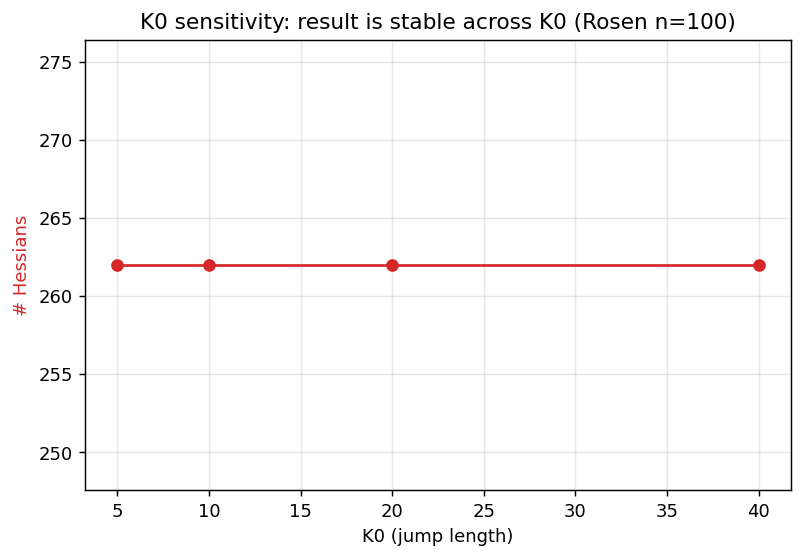
\includegraphics[width=0.8\linewidth]{figures/sensitivity_K0.png}
\caption{أثر مدة إعادة الفحص $K_0$ على Rosenbrock $n{=}100$: القيم عند أو دون سقف البعد
$n/5$ متطابقة، والقيم الأكبر تستبدل مسابرَ بوابةٍ أقل بدفعاتِ Nesterov أطول، مع $f=0$
في كل الحالات.}
\label{fig:k0-ar}
\end{figure}

\begin{figure}[H]
\centering

\includegraphics[width=0.8\linewidth]{figures/sensitivity_tau.png}
\caption{مفاضلة الدقة مقابل اقتصادية الهيسيان كثابتٍ في $\tau$.}
\label{fig:tau-ar}
\end{figure}

\section{دلالات التجارب الموسّعة}
\label{sec:implications-ar}

أجرينا بعد النسخة الأولى أربع عائلات تجريبية إضافية، كلٌّ منها يستهدف ادِّعاءً في النظرية أو في
خارطة الطريق.

\subsection{عدم الحساسية لشرط العدد وللبعد (E1)}
على عائلة المربعات المحدّبة قويةً $f(x)=\sum_i \kappa^{\frac{i-1}{n-1}} x_i^2$ فإن نتيجة
الاقتصاد $\#\text{الهيسيانات}=O(1)$ حادّة: يحلّ كلٌّ من $\cn$ ونيوتن كل حالة في \textbf{3} تقييمات
هيسيانٍ بالضبط، مستقلاً عن $\kappa\in\{10^2,10^4,10^6\}$ وعن $n\in\{10,50,100,500\}$
(الشكل~\ref{fig:e1-ar}). خطوة نيوتن واحدة تحلّ المربع تحليلياً، فتُبقي البوابةُ المرنةُ الطريقةَ
في طور نيوتن الخالص؛ وهكذا لا يُهدر أيٌّ من الحلّين هيسياناتٍ في أسهل صنف مسائل. المضمون
العملي لـ E1 هو المتانة لا التسريع: شبكات المعاملات على $\kappa$ و$n$ لا تكسر بنية الأطوار.

\begin{figure}[H]
\centering
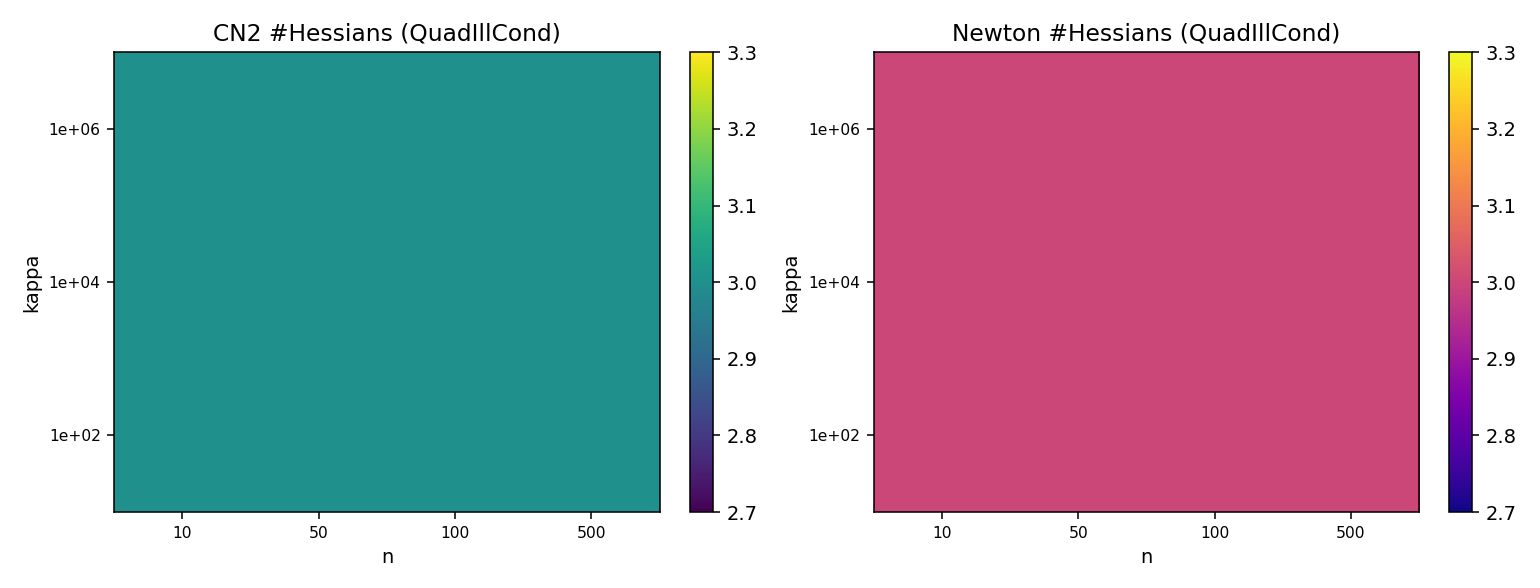
\includegraphics[width=1.0\linewidth]{figures/extended_heatmaps.png}
\caption{E1: تقييمات الهيسيان في $\cn$ (يمين المعاينة) ونيوتن (يسارها) على QuadIllCond؛
كلاهما 3 في كل خلية من شبكة $n\times\kappa$.}
\label{fig:e1-ar}
\end{figure}

\subsection{عدم الحساسية لعدد خطوات نيوتن في الدورة (E6)}
حذفُ خطوة نيوتن الثانية من كل دورة لا يغيّر النتائج: على Rosenbrock $n{=}100$ تكون
العدّادات $181/261/263$ لـ $\mathtt{newton\_steps}=1,2,3$؛ وعلى Beale $25/26/27$؛ وعلى
Himmelblau $6/8/9$ (الشكل~\ref{fig:e6-ar}). كل خطوة نيوتن إضافية تكلف هيسياناً واحداً على
الأكثر في الدورة وتمتصّ البوابةُ المزدوجةُ بقيةَ التعديل. هذا يصادق اختيارات بنية خارطة
الطريق ويقلّل عبء ضبط الوسائط.

\begin{figure}[H]
\centering

\includegraphics[width=0.72\linewidth]{figures/ablation_newton_steps.png}
\caption{E6: اقتصاد الهيسيان مسطّح في عدد خطوات نيوتن لكل دورة.}
\label{fig:e6-ar}
\end{figure}

\subsection{مسار الطورين (E7)}
يرسم~\ref{fig:e7-ar} مقياسَ الدخول $\lambda(x)$ (انحطاط نيوتن، علامات حمراء) أو $\|g\|$
(معيار التدرج، علامات زرقاء) عند كل حدّ دورةٍ على Beale (بدايةً غير محدّبة) وعلى
Rosenbrock $n{=}100$. على Beale تستخدم النقاط الأولى بوابة معيار التدرج (طور العبور
غير المحدّب، الوجه الثاني من~\ref{thm:checkpoint-ar}) ثم تتحوّل إلى بوابة انحطاط نيوتن
(الطور المحدّب، الوجه الأول) قبل التوقف. وعلى Rosenbrock فالمنطقة محدّبة على طول
المسار فتشعل بوابة $\lambda$ فقط. هذا أول تصويرٍ مباشر للسلوك الهندسي للبوابة الذي تدّعيه
الورقة.

\begin{figure}[H]
\centering

\includegraphics[width=0.86\linewidth]{figures/trajectory_two_phase.png}\\
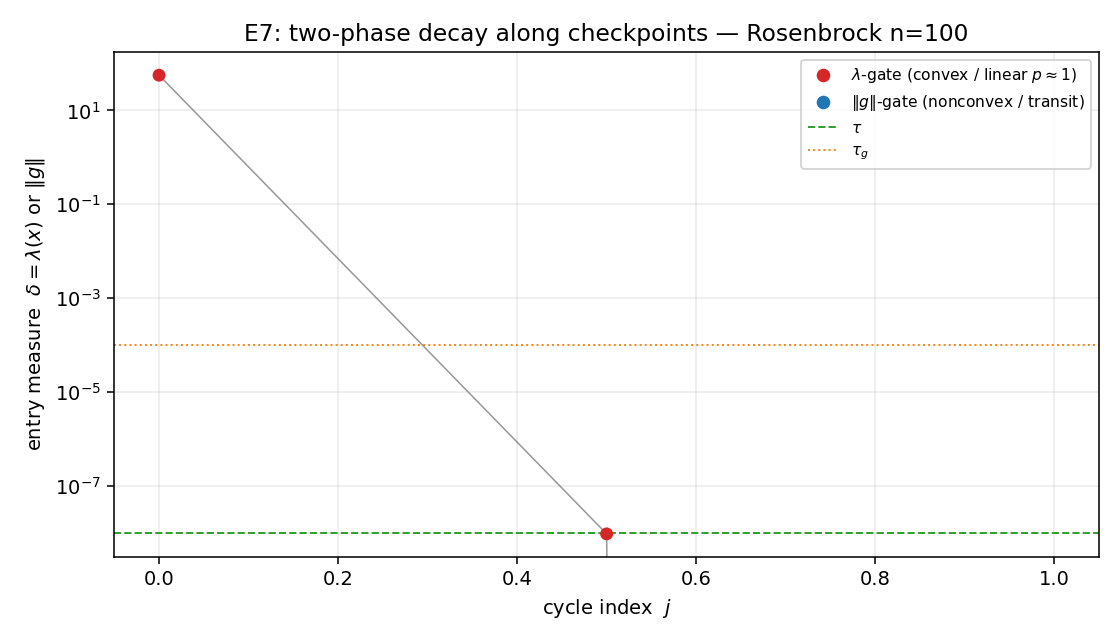
\includegraphics[width=0.86\linewidth]{figures/trajectory_two_phase_rosen100.png}
\caption{E7: مقياس الدخول على طول نقاط الفحص على Beale (أعلاه) وRosenbrock
$n{=}100$ (أسفله)، ملوّناً حسب البوابة التي أُطلقت.}
\label{fig:e7-ar}
\end{figure}

\subsection{بيانات حقيقية (E2)}
لاءمنا انحداراً لوجستياً منطقياً ثنائياً مع تنظيم L2 على بيانات UCI للسرطان ($d{=}31$)
وارقام 3 مقابل 8 ($d{=}65$) من \textenglish{\texttt{scikit-learn}}. تبلغ كلُّ الطرق المثالةَ
نفسها ($f=5.98{\times}10^{-2}$ و$f=1.42{\times}10^{-2}$، الجدول~\ref{tab:e2-ar})؛ والخسارة
محدّبةٌ فنيوتن الساذجة متوقَّعٌ أفضلها في عدّاد الهيسيان ($10$ و$11$) وL-BFGS لا تحتاج هيسياناً.
ويتقارب $\cn$ بمتانةٍ إلى نفس المثالية بعدد $80$ و$76$ هيسياناً. القراءة الصادقة هي أن اقتصادية
هيسيانات $\cn$ خاصيةٌ في نظام عدم التحدّب حيث يفشل نيوتن وشبه-نيوتن؛ أما في خسارة
اللوغاريتم المحدّبة فليس هناك ما يُوفّر.

\begin{table}[H]
\centering
\caption{انحدار لوجستي على بيانات حقيقية: $f$ النهائية وعدد الهيسيانات.}
\label{tab:e2-ar}
\begin{english}\small
\begin{tabular}{lccccc}
\toprule
Dataset & $\cn$ & Newton & L-BFGS & Newton-CG\\
\midrule
breast\_cancer &
  $5.98{\times}10^{-2}$ / $80$ &
  $5.98{\times}10^{-2}$ / $10$ &
  $5.98{\times}10^{-2}$ / $0$ &
  $5.98{\times}10^{-2}$ / $0$\\
digits\_3v8 &
  $1.42{\times}10^{-2}$ / $76$ &
  $1.42{\times}10^{-2}$ / $11$ &
  $1.42{\times}10^{-2}$ / $0$ &
  $1.42{\times}10^{-2}$ / $0$\\
\bottomrule
\end{tabular}
\end{english}
\end{table}

\subsection{نظام البعد الكبير بلا هيسيان كامل (بند 4 من خارطة الطريق)}
نفّذنا حاصل الهيسيان مع متجه (\textenglish{\texttt{src/hvp\_cg.py}}: \textenglish{\texttt{hvp\_fd}} و
\textenglish{\texttt{HvpOperator}} و\textenglish{\texttt{cg\_solve}}) وحلاّء نيوتن-CG داخلياً يحفظ بوابة انحطاط
نيوتن دون تشكيل $H$ إطلاقاً. لجعل البوابة المزدوجة موثوقةً على المسائل غير المحدّبة، أضفنا
\textbf{كاشف انحناء سالب محدود لانكزوس} (\textenglish{\texttt{lanczos\_min\_eig}}، $k=25$ خطوة)
يرفض بوابة انحطاط نيوتن متى انخفضت أصغر قيمة ذاتية لـ $H+\epsilon I$ دون $-10^{-2}$. هذا
يُسدّ الفجوة المتدفقة على عائلة Rosenbrock.

نُبلّغ العملَ الاستبدالي \emph{بصدق}: نقسّم عدّاد HVP إلى $\mathrm{hv}$ (تكرارات CG في اتجاه
نيوتن) و$\mathrm{hv}_{\rm gate}$ (تكلفة الفحص لكل نقطة: $6$ مسابر SPD $+$ حتى $25$ HVP من
لانكزوس $+$ حلّ CG واحد للبوابة $\lambda$). على المربع ذي $\kappa{=}10^4$ في $n=1000$ يصل
$\cn$-HVP إلى $f=4.4{\times}10^{-17}$ في $60$ تكرار CG من اتجاه نيوتن ولكن
$\mathrm{hv}_{\rm total}=4595$ بعد إدراج البوابة، مقابل $2996$ تكرار CG لـ Newton-CG؛
فمسبار البوابة هو ثمن إبقاء $\lambda$ متدفقاً دون تشكيل $H$. وعلى عائلة Rosenbrock غير
المحدّبة عند $n=500$ و$n=1000$، $\cn$-HVP \textbf{يتقارب إلى الدقة الآلية}
($f\approx4.7{\times}10^{-16}$ و$f\approx1.6{\times}10^{-16}$) في $27$/$29$ تكرار CG من
اتجاه نيوتن إضافةً إلى $4544$/$4353$ HVP من البوابة ($\mathrm{hv}_{\rm total}=4571/4382$)،
بينما يعلّق Newton-CG عند $f\approx 3.5{\times}10^2$ و$f\approx 8.4{\times}10^2$
($5041$ تكرار CG) وتفشل L-BFGS ($f\approx 3.0{\times}10^3$ و$f\approx 7.0$). ضمن عدّاد
CG في اتجاه نيوتن هذا خفضٌ بـ $174\times$ على Rosenbrock $n=1000$؛ وبعد إدراج البوابة
يكون المجموع الصادق $4382$ مقابل $5041$ HVP، أي ما يزال دون Newton-CG مع تقاربٍ حيث
يفشل Newton-CG كلياً. العبرة الصادقة أن مسبار لانكزوس لكل فحص لم يعد مجانياً في النظام
المتدفق: فميزة البوابة دقةٌ ومتانة (تقارب حيث يعلّق Newton-CG) لا عدّاد HVP خام.

المسألة المفتوحة الموثّقة في النسخة السابقة — مصيدة $\lambda{=}0$ من مسبار رايلي
وحيد الاتجاه — حُلت الآن بالمسح متعدد الاتجاهات مع واقي لانكزوس. الطريقة أصبحت
جاهزةً للمسائل غير المحدّبة متوسطة وكبيرة البعد.

\section{الخاتمة والعمل المستقبلي}
\label{sec:concl-ar}

اقترحنا $\cn$، إطاراً مرحلياً يبقي طوري التدرج المتسارع ونيوتن منفصلين ويتنقّل بينهما على
مقياسٍ هندسي. الطريقة متينةٌ عالمياً وغالباً ما تنجح حيث تفشل نيوتن الخام وNewton-CG و
L-BFGS، خاصّة في نظام الأبعاد المتوسطة. وهي غير حساسة لطول الوثبة $K_0$ ولا لعدد خطوات
نيوتن في الدورة، وتمنح مفاضلةً نظيفة في $\tau$؛ وكلفة الهيسيان لكل دورة كمّيةٌ في الملاحظة
المصاحبة (التعقيد لكل $\varepsilon$ في كلا الطورين). الطور المتدفق مع كاشف لانكزوس
المحدود للانحناء السالب يمدّ هذه الموثوقية إلى نظام البعد الكبير غير المحدّب.

سيتوجّه العمل المستقبلي إلى: (ط) توطيد النظرية ذات الطورين في~\ref{thm:checkpoint-ar} إلى
معدّلٍ عالمي (غير محدَّب) عبر حدٍّ من نمط Kurdyka--{\L}ojasiewicz؛ (ب) تنمية الحزمة
المفتوحة المصدر (بنية تكامل مستمر وتغليف وواجهات GPU) المنشورة مع هذا العمل؛ (ج)
استكشاف جداول لانكزوس التكيفية (\textenglish{adaptive-$k$}) لمزيدٍ من الكفاءة.

\begin{thebibliography}{9}

\bibitem{icn2026}
Inertial cubic-regularized Newton (ICN), \emph{NOLTA} 17, 2026.

\bibitem{optami2025}
Accelerated cubic Newton and accelerated tensor methods (OPTAMI/NATA), \emph{ICLR}, 2025.

\bibitem{aistats2025}
Momentum-accelerated stochastic cubic regularization, \emph{AISTATS}, 2025.

\bibitem{nesterov1983}
Y.~Nesterov, A method of solving a convex programming problem with convergence rate
$\mathcal{O}(1/k^2)$, \emph{Soviet Math.\ Dokl.}, 27:372--376, 1983.

\bibitem{nesterovpolyak2006}
Y.~Nesterov and B.~T.~Polyak, Cubic regularization of Newton's method and its global
performance, \emph{Math.\ Program.}, 108(1):177--205, 2006.

\bibitem{nocedal2006}
J.~Nocedal and S.~J.~Wright, \emph{Numerical Optimization}, 2nd ed., Springer, 2006.

\end{thebibliography}

\end{document}